%==============================================================================
% MSI-Seminar WS 2026/27, Vision-Language-Action-Modelle in der Robotik
% Team 3: Daten, Skalierung und Open-World-Generalisierung
%
% IEEEtran journal template (IEEE Transactions, as used by T-ASE).
% Build: make  (or latexmk -pdf main.tex, or upload to Overleaf)
%==============================================================================
\documentclass[lettersize,journal]{IEEEtran}

\usepackage{amsmath,amsfonts,amssymb}
\usepackage{array}
\usepackage{booktabs}
\usepackage{multirow}
\usepackage{tabularx}
\usepackage{textcomp}
\usepackage{stfloats}
\usepackage{url}
\usepackage{graphicx}
\usepackage{cite}
\usepackage{algorithm}
\usepackage{algorithmic}
\usepackage[caption=false,font=normalsize,labelfont=sf,textfont=sf]{subfig}
\usepackage[dvipsnames]{xcolor}
\usepackage{siunitx}
\sisetup{per-mode=symbol}
\usepackage[hidelinks]{hyperref}

\graphicspath{{figures/}}

%--- Platzhalter, vor der Abgabe alle entfernen (make check) --------------------
\newcommand{\TODO}[1]{\textcolor{red}{[TODO: #1]}}

\begin{document}
\bstctlcite{IEEEexample:BSTcontrol} % more than six authors -> first author et al.

% Arbeitstitel, darf geändert werden
\title{Data, Scale, and Open-World Generalization\\in VLA Models}

\author{First~Author and Second~Author%
\thanks{The authors are with the University of Applied Sciences (HTWG) Konstanz, 78462 Konstanz, Germany.}}

\markboth{MSI Seminar ``Vision-Language-Action Models in Robotics'', HTWG Konstanz, Winter Term 2026/27}%
{Team 3: Data and Generalization}

\maketitle

\begin{abstract}
% 150--250 Wörter: Thema, Leitfrage, betrachtete Arbeiten, wichtigste Ergebnisse.
% Zuletzt schreiben.
\TODO{Abstract, 150--250 words.}
\end{abstract}

\begin{IEEEkeywords}
Vision-language-action models, robot learning, \TODO{3--5 further keywords}.
\end{IEEEkeywords}

\section{Introduction}
\label{sec:introduction}
% Leitfrage des Blocks: Welche Daten machen ein VLA generalisierbar, und wie verhindert man, dass das VLM sein Weltwissen verliert?

\TODO{Introduction. Guiding question of the block: ``Which data make a VLA generalize, and how do we keep the VLM from losing its world knowledge?'' Core papers: \cite{oxe2023,khazatsky2024droid,pi2025pi05,driess2025ki}.}

% Beispiele für die üblichen Elemente im IEEE-Stil, angelehnt an das IEEE-Journal-Template
% (bare_jrnl_new_sample4.tex). Dient als Vorlage: diesen Abschnitt durch die eigenen Abschnitte
% ersetzen (als eigene Dateien unter sections/, in main.tex einbinden) und dann löschen.

\section{Examples of Common Elements}
\label{sec:examples}

\TODO{Replace this section with your own sections.}

\subsection{Sections and Subsections}
Primary headings use Roman numerals, secondary headings capital letters, and tertiary headings Arabic numerals. Refer to sections as Section~\ref{sec:introduction}.

\subsubsection{Tertiary Heading}
Use tertiary headings sparingly in a six-page paper.

\subsection{Citations}
Cite with \verb|\cite{key}|, e.g., \cite{oxe2023}, and several references in one bracket as \cite{oxe2023,khazatsky2024droid}. All entries live in \texttt{refs.bib}. The reference list is generated in IEEE style, and only cited entries appear in it. Name authors in the text with ``et al.'' when a reference has three or more authors.

\subsection{Lists}
A bulleted list:
\begin{itemize}
  \item first item;
  \item second item.
\end{itemize}
A numbered list:
\begin{enumerate}
  \item first step;
  \item second step.
\end{enumerate}

\subsection{Equations}
Number display equations, punctuate them as part of the sentence, and refer to them as (\ref{eq:example}). A policy that predicts a chunk of $H$ actions from the observation $\mathbf{o}_t$ and the instruction $\ell$ can be written as
\begin{equation}
  \mathbf{A}_t = \left[\mathbf{a}_t, \mathbf{a}_{t+1}, \dots, \mathbf{a}_{t+H-1}\right] \sim \pi_\theta\left(\cdot \mid \mathbf{o}_t, \ell\right).
  \label{eq:example}
\end{equation}
Use \texttt{align} for multi-line equations, aligned at the relation sign:
\begin{align}
  y &= a x + b \label{eq:example_line1}\\
    &= a \left(x + \frac{b}{a}\right). \label{eq:example_line2}
\end{align}
Write units with \texttt{siunitx}, e.g., \SI{50}{\hertz} or \SI{0.5}{\meter\per\second}.

\subsection{Figures}
Place figure files in \texttt{figures/}, preferably as vector graphics (PDF), and refer to them as Fig.~\ref{fig:example}. Captions go below the figure. For a figure taken from a paper, state the source in the caption, e.g., ``Adapted from~\cite{oxe2023}.'' Plots made with Python use the shared style \texttt{figures/ieee.mplstyle}, which sets the body font (Times, \SI{10}{pt}), the column width, and the \texttt{tab20c} colors; \texttt{figures/example\_plot.py} creates Fig.~\ref{fig:example}.

\begin{figure}[t]
  \centering
  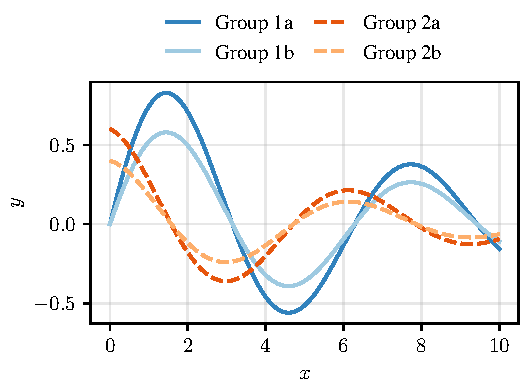
\includegraphics[width=\columnwidth]{example_plot}
  \caption{Example of a single-column figure. One hue per group and lighter shades for variants (\texttt{tab20c}). Captions end with a period.}
  \label{fig:example}
\end{figure}

Figures with several parts use \verb|\subfloat| and describe the parts in the main caption, as in Fig.~\ref{fig:example_wide}.

\begin{figure*}[t]
  \centering
  \subfloat[]{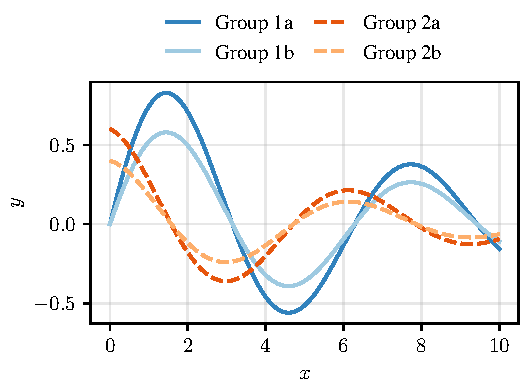
\includegraphics[width=0.45\textwidth]{example_plot}\label{fig:example_a}}
  \hfil
  \subfloat[]{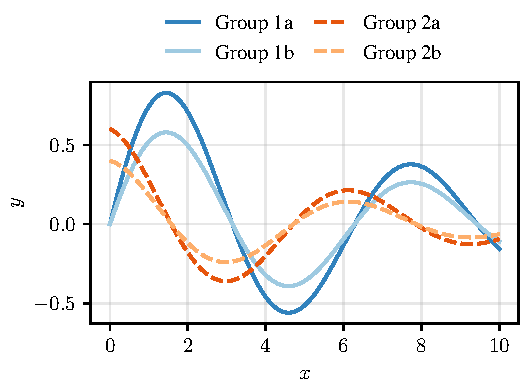
\includegraphics[width=0.45\textwidth]{example_plot}\label{fig:example_b}}
  \caption{Example of a figure spanning both columns. (a) First case. (b) Second case.}
  \label{fig:example_wide}
\end{figure*}

% Abbildungen und Tabellen über beide Spalten (figure*, table*) erscheinen frühestens oben auf der
% nächsten Seite. Deshalb im Quelltext etwas vor der Stelle einbinden, an der sie besprochen werden.
% Tabelle über beide Spalten: table* und tabularx mit \textwidth.
% X-Spalten brechen langen Text um. Im Text: Table~\ref{tab:example_wide}.
\begin{table*}[t]
  \centering
  \caption{An Example of a Table Spanning Both Columns}
  \label{tab:example_wide}
  \footnotesize
  \begin{tabularx}{\textwidth}{@{}l>{\raggedright\arraybackslash}X>{\raggedright\arraybackslash}X@{}}
    \toprule
    Aspect & Column With Longer Text & Another Column With Longer Text \\
    \midrule
    Row 1 & Text in X columns wraps automatically to the available width. & -- \\
    Row 2 & -- & -- \\
    \bottomrule
  \end{tabularx}
\end{table*}


\subsection{Tables}
Table captions use title case and go above the table. Table~\ref{tab:example_wide} spans both columns, Table~\ref{tab:example} one column. Each table lives in its own file in \texttt{tables/}.

% Tabelle über eine Spalte, Stil wie im T-ASE-Paper: Caption in Title Case ÜBER der Tabelle,
% \label nach \caption, \footnotesize, booktabs-Linien (keine senkrechten Linien), -- für leere Zellen,
% Anmerkungen klein unter der Tabelle. Im Text: Table~\ref{tab:example}.
\begin{table}[t]
  \centering
  \caption{An Example of a Table}
  \label{tab:example}
  \footnotesize
  \begin{tabular}{@{}lccc@{}}
    \toprule
     & \multicolumn{2}{c}{Grouped Columns} & \\
    \cmidrule(lr){2-3}
    Paper & Column A & Column B & Column C \\
    \midrule
    Open X-Embodiment~\cite{oxe2023} & -- & -- & -- \\
    DROID~\cite{khazatsky2024droid} & -- & -- & -- \\
    $\pi_{0.5}$~\cite{pi2025pi05} & -- & -- & -- \\
    Knowledge Insulation~\cite{driess2025ki} & -- & -- & -- \\
    \bottomrule
  \end{tabular}
  \\[2pt]\raggedright\scriptsize Notes below the table, e.g., abbreviations. --: not reported.
\end{table}


\subsection{Algorithms}
Algorithms are numbered and have a short title, see Algorithm~\ref{alg:example}.

\begin{algorithm}[t]
  \caption{Example of an Algorithm}
  \label{alg:example}
  \begin{algorithmic}[1]
    \REQUIRE policy $\pi_\theta$, instruction $\ell$, chunk length $H$
    \WHILE{task not finished}
      \STATE observe $\mathbf{o}_t$
      \STATE $\mathbf{A}_t \gets \pi_\theta(\mathbf{o}_t, \ell)$ \hfill (\ref{eq:example})
      \FOR{$k = 0$ \TO $H-1$}
        \STATE execute $\mathbf{a}_{t+k}$
      \ENDFOR
    \ENDWHILE
  \end{algorithmic}
\end{algorithm}

\section{Conclusion}
\label{sec:conclusion}

\TODO{Conclusion.}

% Unnummerierter Abschnitt direkt vor der Literatur (IEEE).
% Hier angeben, welche KI-Werkzeuge (Name, Version) wofür genutzt wurden, z.B. Literaturrecherche,
% Zusammenfassen von Papers, Übersetzung, Sprachkorrektur, Textentwurf, Abbildungen, Code.
% Dazu die betroffenen Abschnitte und den Umfang nennen. Wurden keine KI-Werkzeuge genutzt,
% dies ebenfalls angeben. IEEE verlangt diese Angabe im Acknowledgment; KI-Werkzeuge sind keine
% Autoren, die Verantwortung für den gesamten Inhalt liegt bei den Autoren.

\section*{Acknowledgment}
\TODO{State which AI tools (name and version) were used, for what, in which sections, and to what extent, e.g., ``[Tool, version] was used to improve the grammar of Sections~II and~III. All content was checked by the authors.'' If no AI tools were used, state this.}


\bibliographystyle{IEEEtran}
\bibliography{refs}

\end{document}
